\documentclass[twoside]{book}

% Packages required by doxygen
\usepackage{fixltx2e}
\usepackage{calc}
\usepackage{doxygen}
\usepackage[export]{adjustbox} % also loads graphicx
\usepackage{graphicx}
\usepackage[utf8]{inputenc}
\usepackage{makeidx}
\usepackage{multicol}
\usepackage{multirow}
\PassOptionsToPackage{warn}{textcomp}
\usepackage{textcomp}
\usepackage[nointegrals]{wasysym}
\usepackage[table]{xcolor}

% Font selection
\usepackage[T1]{fontenc}
\usepackage[scaled=.90]{helvet}
\usepackage{courier}
\usepackage{amssymb}
\usepackage{sectsty}
\renewcommand{\familydefault}{\sfdefault}
\allsectionsfont{%
  \fontseries{bc}\selectfont%
  \color{darkgray}%
}
\renewcommand{\DoxyLabelFont}{%
  \fontseries{bc}\selectfont%
  \color{darkgray}%
}
\newcommand{\+}{\discretionary{\mbox{\scriptsize$\hookleftarrow$}}{}{}}

% Page & text layout
\usepackage{geometry}
\geometry{%
  a4paper,%
  top=2.5cm,%
  bottom=2.5cm,%
  left=2.5cm,%
  right=2.5cm%
}
\tolerance=750
\hfuzz=15pt
\hbadness=750
\setlength{\emergencystretch}{15pt}
\setlength{\parindent}{0cm}
\setlength{\parskip}{3ex plus 2ex minus 2ex}
\makeatletter
\renewcommand{\paragraph}{%
  \@startsection{paragraph}{4}{0ex}{-1.0ex}{1.0ex}{%
    \normalfont\normalsize\bfseries\SS@parafont%
  }%
}
\renewcommand{\subparagraph}{%
  \@startsection{subparagraph}{5}{0ex}{-1.0ex}{1.0ex}{%
    \normalfont\normalsize\bfseries\SS@subparafont%
  }%
}
\makeatother

% Headers & footers
\usepackage{fancyhdr}
\pagestyle{fancyplain}
\fancyhead[LE]{\fancyplain{}{\bfseries\thepage}}
\fancyhead[CE]{\fancyplain{}{}}
\fancyhead[RE]{\fancyplain{}{\bfseries\leftmark}}
\fancyhead[LO]{\fancyplain{}{\bfseries\rightmark}}
\fancyhead[CO]{\fancyplain{}{}}
\fancyhead[RO]{\fancyplain{}{\bfseries\thepage}}
\fancyfoot[LE]{\fancyplain{}{}}
\fancyfoot[CE]{\fancyplain{}{}}
\fancyfoot[RE]{\fancyplain{}{\bfseries\scriptsize Generated by Doxygen }}
\fancyfoot[LO]{\fancyplain{}{\bfseries\scriptsize Generated by Doxygen }}
\fancyfoot[CO]{\fancyplain{}{}}
\fancyfoot[RO]{\fancyplain{}{}}
\renewcommand{\footrulewidth}{0.4pt}
\renewcommand{\chaptermark}[1]{%
  \markboth{#1}{}%
}
\renewcommand{\sectionmark}[1]{%
  \markright{\thesection\ #1}%
}

% Indices & bibliography
\usepackage{natbib}
\usepackage[titles]{tocloft}
\setcounter{tocdepth}{3}
\setcounter{secnumdepth}{5}
\makeindex

% Hyperlinks (required, but should be loaded last)
\usepackage{ifpdf}
\ifpdf
  \usepackage[pdftex,pagebackref=true]{hyperref}
\else
  \usepackage[ps2pdf,pagebackref=true]{hyperref}
\fi
\hypersetup{%
  colorlinks=true,%
  linkcolor=blue,%
  citecolor=blue,%
  unicode%
}

% Custom commands
\newcommand{\clearemptydoublepage}{%
  \newpage{\pagestyle{empty}\cleardoublepage}%
}

\usepackage{caption}
\captionsetup{labelsep=space,justification=centering,font={bf},singlelinecheck=off,skip=4pt,position=top}

%===== C O N T E N T S =====

\begin{document}

% Titlepage & ToC
\hypersetup{pageanchor=false,
             bookmarksnumbered=true,
             pdfencoding=unicode
            }
\pagenumbering{alph}
\begin{titlepage}
\vspace*{7cm}
\begin{center}%
{\Large My Project }\\
\vspace*{1cm}
{\large Generated by Doxygen 1.8.13}\\
\end{center}
\end{titlepage}
\clearemptydoublepage
\pagenumbering{roman}
\tableofcontents
\clearemptydoublepage
\pagenumbering{arabic}
\hypersetup{pageanchor=true}

%--- Begin generated contents ---
\chapter{My Personal Index Page}
\label{index}\hypertarget{index}{}\hypertarget{index_intro_sec}{}\section{Introduction}\label{index_intro_sec}
This is the introduction. Hello world! This is Jingyi\textquotesingle{}s first Doxygen file! 
\chapter{Class Index}
\section{Class List}
Here are the classes, structs, unions and interfaces with brief descriptions\+:\begin{DoxyCompactList}
\item\contentsline{section}{\hyperlink{classBus}{Bus} \\*As the description mentioned above, \hyperlink{classBus}{Bus} Factory was created to generate different types of buses. So, in this class, I implimented three different buses categorized by capacity of the bus, small, regular, and large. Small bus will have 30 maximum capacity, regular is assigned with 60 capacity while large can load 90 passengers maximum. The three class all inherited from their parent class, \hyperlink{classBus}{Bus}. Also, they all have on public class, Report, to tell people which type of bus is generated when the simulator is running }{\pageref{classBus}}{}
\item\contentsline{section}{\hyperlink{classBusFactory}{Bus\+Factory} \\*To make the project more releastic, I implemented a new class, \hyperlink{classBus}{Bus} Factory, which can generate different kinds of buses. So far, the needs for different buses types are just reporting different capacity. So, here I used concreate factory method for bus factory. The class basically just generate the bus and use an int parameter to define the type of the buses. When the parameter is set to one, small bus will be generated, regular size will be generated when 2 is assigned to the parameter and leaves value 3 for having large size bus. The value will be assigned randomly to make sure all kinds of buses will appear on the simulator. The process will be applied in visualization\+\_\+simulator }{\pageref{classBusFactory}}{}
\item\contentsline{section}{\hyperlink{classLargeBus}{Large\+Bus} \\*A Small \hyperlink{classBus}{Bus} product, bus size is 90 maximum capacity }{\pageref{classLargeBus}}{}
\item\contentsline{section}{\hyperlink{classRegularBus}{Regular\+Bus} \\*A Small \hyperlink{classBus}{Bus} product, bus size is 60 maximum capacity }{\pageref{classRegularBus}}{}
\item\contentsline{section}{\hyperlink{classSmallBus}{Small\+Bus} \\*A Small \hyperlink{classBus}{Bus} product, bus size is 30 maximum capacity }{\pageref{classSmallBus}}{}
\item\contentsline{section}{\hyperlink{classVisualizationSimulator}{Visualization\+Simulator} \\*The pause functionality mainly rely on Update(). Because, when the simulator is paused, we want the simulator to stop updating. So, by defining the status of pause button (clicked or not clicked), Update() will make a decision to keep updating or pause the process. The similar logic also works for resume functionality. If pause function is called, then un-\/pause it, or pause the function if the pause function is not called }{\pageref{classVisualizationSimulator}}{}
\end{DoxyCompactList}

\chapter{File Index}
\section{File List}
Here is a list of all documented files with brief descriptions\+:\begin{DoxyCompactList}
\item\contentsline{section}{/home/jinxx679/\+Documents/3081/repo-\/jinxx679/project/src/\hyperlink{bus_8cc}{bus.\+cc} }{\pageref{bus_8cc}}{}
\item\contentsline{section}{/home/jinxx679/\+Documents/3081/repo-\/jinxx679/project/src/\hyperlink{bus_8h}{bus.\+h} }{\pageref{bus_8h}}{}
\item\contentsline{section}{/home/jinxx679/\+Documents/3081/repo-\/jinxx679/project/src/\hyperlink{bus__factory_8h}{bus\+\_\+factory.\+h} }{\pageref{bus__factory_8h}}{}
\item\contentsline{section}{/home/jinxx679/\+Documents/3081/repo-\/jinxx679/project/src/{\bfseries mainpage.\+h} }{\pageref{mainpage_8h}}{}
\item\contentsline{section}{/home/jinxx679/\+Documents/3081/repo-\/jinxx679/project/web\+\_\+code/web/{\bfseries visualization\+\_\+simulator.\+h} }{\pageref{visualization__simulator_8h}}{}
\end{DoxyCompactList}

\chapter{Class Documentation}
\hypertarget{classPassenger}{}\section{Passenger Class Reference}
\label{classPassenger}\index{Passenger@{Passenger}}


The main class for the generation of useful information.  




{\ttfamily \#include $<$passenger.\+h$>$}



Collaboration diagram for Passenger\+:\nopagebreak
\begin{figure}[H]
\begin{center}
\leavevmode
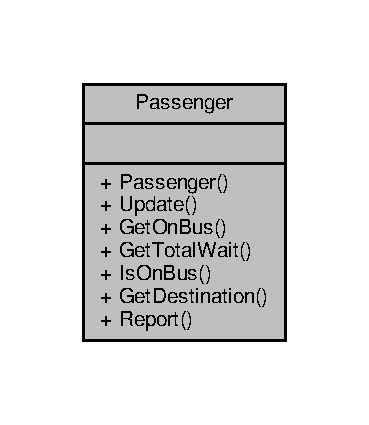
\includegraphics[width=177pt]{classPassenger__coll__graph}
\end{center}
\end{figure}
\subsection*{Public Member Functions}
\begin{DoxyCompactItemize}
\item 
\mbox{\Hypertarget{classPassenger_a5c3addb9a6fd03e5e5642ed844e2702c}\label{classPassenger_a5c3addb9a6fd03e5e5642ed844e2702c}} 
{\bfseries Passenger} (int=-\/1, std\+::string=\char`\"{}Nobody\char`\"{})
\item 
\mbox{\Hypertarget{classPassenger_a960de3b29fc17a2c2d79c0b79d5cf299}\label{classPassenger_a960de3b29fc17a2c2d79c0b79d5cf299}} 
void {\bfseries Update} ()
\item 
\mbox{\Hypertarget{classPassenger_ae2ba639cfef39781ac079778578bd9fe}\label{classPassenger_ae2ba639cfef39781ac079778578bd9fe}} 
void {\bfseries Get\+On\+Bus} ()
\item 
\mbox{\Hypertarget{classPassenger_a25158560f790ef7ef06d94c414b34f25}\label{classPassenger_a25158560f790ef7ef06d94c414b34f25}} 
int {\bfseries Get\+Total\+Wait} () const
\item 
\mbox{\Hypertarget{classPassenger_a2acf008ec444afcc859b914ee24add0e}\label{classPassenger_a2acf008ec444afcc859b914ee24add0e}} 
bool {\bfseries Is\+On\+Bus} () const
\item 
int \hyperlink{classPassenger_a49db0ee527377aae6077df190a11501c}{Get\+Destination} () const
\begin{DoxyCompactList}\small\item\em Generation of a stop id set by passenger. \end{DoxyCompactList}\item 
\mbox{\Hypertarget{classPassenger_ac54ce797e412a4895febe10f07dc5df5}\label{classPassenger_ac54ce797e412a4895febe10f07dc5df5}} 
void {\bfseries Report} () const
\end{DoxyCompactItemize}


\subsection{Detailed Description}
The main class for the generation of useful information. 

Functions for passengers to set their travel information. 

\subsection{Member Function Documentation}
\mbox{\Hypertarget{classPassenger_a49db0ee527377aae6077df190a11501c}\label{classPassenger_a49db0ee527377aae6077df190a11501c}} 
\index{Passenger@{Passenger}!Get\+Destination@{Get\+Destination}}
\index{Get\+Destination@{Get\+Destination}!Passenger@{Passenger}}
\subsubsection{\texorpdfstring{Get\+Destination()}{GetDestination()}}
{\footnotesize\ttfamily int Passenger\+::\+Get\+Destination (\begin{DoxyParamCaption}{ }\end{DoxyParamCaption}) const}



Generation of a stop id set by passenger. 

This function will be used to get the stop id of passenger\textquotesingle{}s destination. 

The documentation for this class was generated from the following files\+:\begin{DoxyCompactItemize}
\item 
/home/jinxx679/\+Documents/repo-\/jinxx679/repo-\/jinxx679/labs/lab07\+\_\+style\+\_\+doxy/src/passenger.\+h\item 
/home/jinxx679/\+Documents/repo-\/jinxx679/repo-\/jinxx679/labs/lab07\+\_\+style\+\_\+doxy/src/passenger.\+cc\end{DoxyCompactItemize}

\hypertarget{classPassengerFactory}{}\section{Passenger\+Factory Class Reference}
\label{classPassengerFactory}\index{Passenger\+Factory@{Passenger\+Factory}}


Collaboration diagram for Passenger\+Factory\+:\nopagebreak
\begin{figure}[H]
\begin{center}
\leavevmode
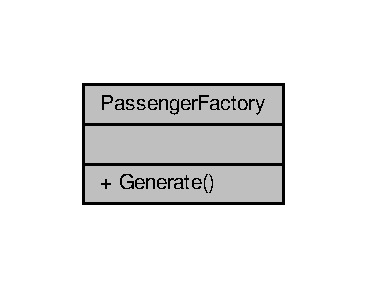
\includegraphics[width=176pt]{classPassengerFactory__coll__graph}
\end{center}
\end{figure}
\subsection*{Static Public Member Functions}
\begin{DoxyCompactItemize}
\item 
\mbox{\Hypertarget{classPassengerFactory_a2952ba78ceb285f445bc768d287230d2}\label{classPassengerFactory_a2952ba78ceb285f445bc768d287230d2}} 
static \hyperlink{classPassenger}{Passenger} $\ast$ {\bfseries Generate} (int, int)
\end{DoxyCompactItemize}


The documentation for this class was generated from the following files\+:\begin{DoxyCompactItemize}
\item 
/home/jinxx679/\+Documents/3081/repo-\/jinxx679/project/src/\hyperlink{passenger__factory_8h}{passenger\+\_\+factory.\+h}\item 
/home/jinxx679/\+Documents/3081/repo-\/jinxx679/project/src/\hyperlink{passenger__factory_8cc}{passenger\+\_\+factory.\+cc}\end{DoxyCompactItemize}

\chapter{File Documentation}
\hypertarget{main_8cc}{}\section{/home/jinxx679/\+Documents/repo-\/jinxx679/repo-\/jinxx679/labs/lab07\+\_\+style\+\_\+doxy/src/main.cc File Reference}
\label{main_8cc}\index{/home/jinxx679/\+Documents/repo-\/jinxx679/repo-\/jinxx679/labs/lab07\+\_\+style\+\_\+doxy/src/main.\+cc@{/home/jinxx679/\+Documents/repo-\/jinxx679/repo-\/jinxx679/labs/lab07\+\_\+style\+\_\+doxy/src/main.\+cc}}
{\ttfamily \#include $<$iostream$>$}\newline
{\ttfamily \#include $<$vector$>$}\newline
{\ttfamily \#include \char`\"{}src/passenger.\+h\char`\"{}}\newline
Include dependency graph for main.\+cc\+:\nopagebreak
\begin{figure}[H]
\begin{center}
\leavevmode
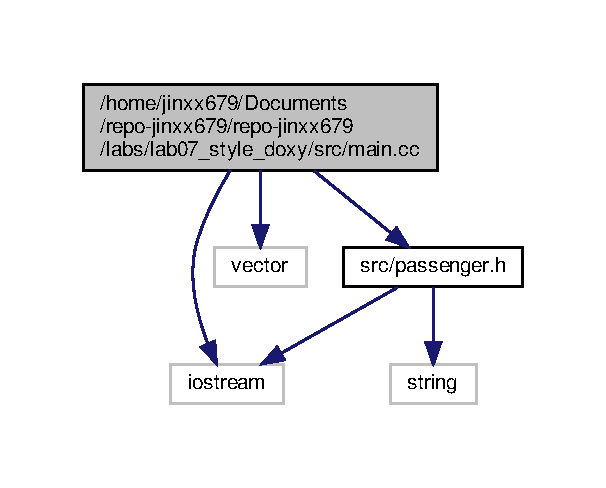
\includegraphics[width=291pt]{main_8cc__incl}
\end{center}
\end{figure}
\subsection*{Functions}
\begin{DoxyCompactItemize}
\item 
\mbox{\Hypertarget{main_8cc_ae66f6b31b5ad750f1fe042a706a4e3d4}\label{main_8cc_ae66f6b31b5ad750f1fe042a706a4e3d4}} 
int {\bfseries main} ()
\end{DoxyCompactItemize}


\subsection{Detailed Description}
\begin{DoxyCopyright}{Copyright}
2019 3081 Staff, All rights reserved. 
\end{DoxyCopyright}

\hypertarget{passenger__factory_8cc}{}\section{/home/jinxx679/\+Documents/3081/repo-\/jinxx679/project/src/passenger\+\_\+factory.cc File Reference}
\label{passenger__factory_8cc}\index{/home/jinxx679/\+Documents/3081/repo-\/jinxx679/project/src/passenger\+\_\+factory.\+cc@{/home/jinxx679/\+Documents/3081/repo-\/jinxx679/project/src/passenger\+\_\+factory.\+cc}}
{\ttfamily \#include $<$random$>$}\newline
{\ttfamily \#include $<$string$>$}\newline
{\ttfamily \#include \char`\"{}src/passenger\+\_\+factory.\+h\char`\"{}}\newline
Include dependency graph for passenger\+\_\+factory.\+cc\+:\nopagebreak
\begin{figure}[H]
\begin{center}
\leavevmode
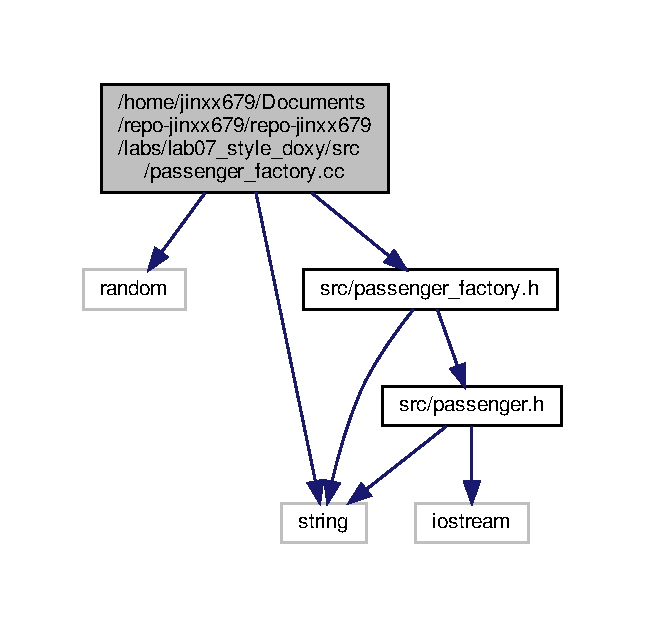
\includegraphics[width=310pt]{passenger__factory_8cc__incl}
\end{center}
\end{figure}
\subsection*{Functions}
\begin{DoxyCompactItemize}
\item 
\mbox{\Hypertarget{passenger__factory_8cc_af34adcff7354e7e8d172f7a97bc05d68}\label{passenger__factory_8cc_af34adcff7354e7e8d172f7a97bc05d68}} 
std\+::mt19937 {\bfseries e} (dev())
\item 
\mbox{\Hypertarget{passenger__factory_8cc_a1d818b31bbf5715a76ee321d8a0993e0}\label{passenger__factory_8cc_a1d818b31bbf5715a76ee321d8a0993e0}} 
std\+::uniform\+\_\+int\+\_\+distribution$<$ std\+::mt19937\+::result\+\_\+type $>$ {\bfseries dist} (1, 1000)
\end{DoxyCompactItemize}
\subsection*{Variables}
\begin{DoxyCompactItemize}
\item 
\mbox{\Hypertarget{passenger__factory_8cc_ad768868c172722a84c70801c1382438f}\label{passenger__factory_8cc_ad768868c172722a84c70801c1382438f}} 
std\+::random\+\_\+device {\bfseries dev}
\end{DoxyCompactItemize}


\subsection{Detailed Description}
\begin{DoxyCopyright}{Copyright}
2019 3081 Staff, All rights reserved. 
\end{DoxyCopyright}

\hypertarget{passenger__factory_8h}{}\section{/home/jinxx679/\+Documents/3081/repo-\/jinxx679/project/src/passenger\+\_\+factory.h File Reference}
\label{passenger__factory_8h}\index{/home/jinxx679/\+Documents/3081/repo-\/jinxx679/project/src/passenger\+\_\+factory.\+h@{/home/jinxx679/\+Documents/3081/repo-\/jinxx679/project/src/passenger\+\_\+factory.\+h}}
{\ttfamily \#include $<$string$>$}\newline
{\ttfamily \#include \char`\"{}src/passenger.\+h\char`\"{}}\newline
Include dependency graph for passenger\+\_\+factory.\+h\+:\nopagebreak
\begin{figure}[H]
\begin{center}
\leavevmode
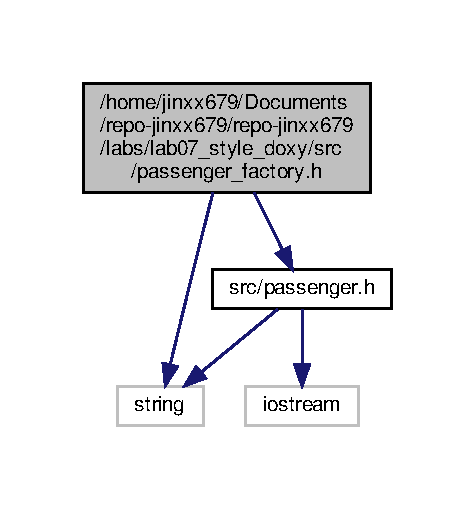
\includegraphics[width=227pt]{passenger__factory_8h__incl}
\end{center}
\end{figure}
This graph shows which files directly or indirectly include this file\+:\nopagebreak
\begin{figure}[H]
\begin{center}
\leavevmode
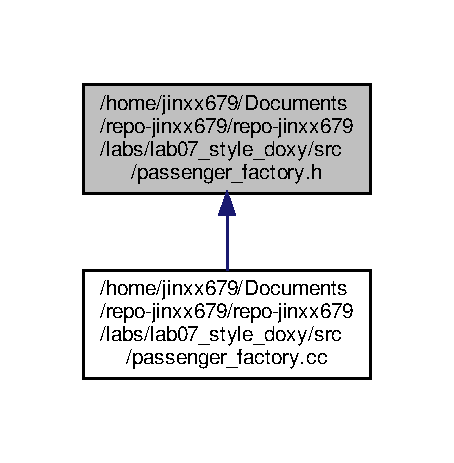
\includegraphics[width=350pt]{passenger__factory_8h__dep__incl}
\end{center}
\end{figure}
\subsection*{Classes}
\begin{DoxyCompactItemize}
\item 
class \hyperlink{classPassengerFactory}{Passenger\+Factory}
\end{DoxyCompactItemize}


\subsection{Detailed Description}
\begin{DoxyCopyright}{Copyright}
2019 3081 Staff, All rights reserved. 
\end{DoxyCopyright}

%--- End generated contents ---

% Index
\backmatter
\newpage
\phantomsection
\clearemptydoublepage
\addcontentsline{toc}{chapter}{Index}
\printindex

\end{document}
